%%=============================================================================
%% Opstellen projecten
%%=============================================================================

\chapter{Aanmaken blanco project}%
\label{ch:projecten}

Na het opzetten van de ontwikkelomgeving voor zowel native als cross-platform gaan 
we een project opstellen dat we als basis zullen nemen om de functionaliteiten te 
implementeren. In dit hoofdstuk wordt uitgelegd hoe dat gebeurt.

\section{Android Studio}
Bij Android Studio kunnen we in de IDE zelf nieuwe projecten aanmaken om de 
functionaliteiten te maken. Dit doen we met \textit{File > New > New Project...}. 
Hierna krijgen we een overzicht van projecten die we als basis kunnen gebruiken. Ook 
kan er op dit scherm gekozen worden voor welk apparaat de applicatie is.
\begin{figure}[H]
    \centering
    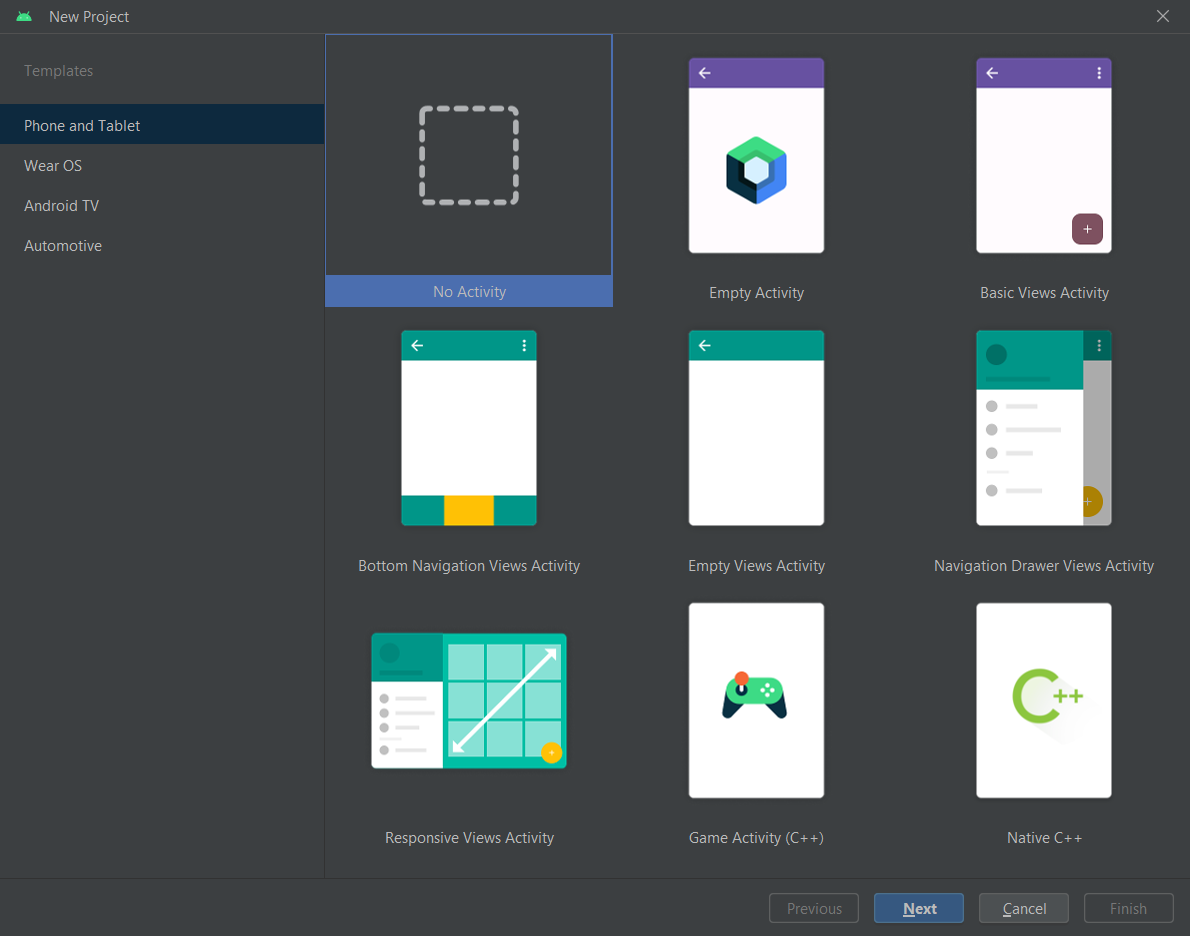
\includegraphics[height=0.35\textheight]{OverzichtProjecten.png}
    \caption{Overzicht startprojecten Android Studio.}
\end{figure}
Afhankelijk van de functionaliteit dat we gaan implementeren zullen we dus andere 
startprojecten kunnen kiezen. Na het kiezen van het startproject geven we een naam, 
programmeertaal en de minimaal ondersteunde Android API. Voor dit onderzoek kiezen we 
voor Kotlin. De naam en minimale ondersteunde Android API speelt hierbij geen rol.

\subsection{Basisfunctionaliteiten}
\label{par:basisfunctionaliteiten}
Bij de basisfunctionaliteiten zullen we als startproject 
\textbf{Bottom Navigation Views Activity} gebruiken om te kunnen navigeren tussen 
verschillende schermen. Daardoor moeten we zelf geen extra libraries gaan implementeren.

\subsection{Overige functionaliteiten}
Voor de overige functionaliteiten (gebruik van sensoren, 
push-notificaties en audio- en videospelers) zullen we als startproject 
\textbf{Empty Activity} gebruiken. Op die manier hebben we de minste \gls{overhead} 
dat de resultaten kan beïnvloeden.

\subsection{Firebase Performance Monitoring}
Om de performantie de applicaties te meten moeten we de Firebase Performance Monitoring tool 
in het project implementeren. 

\paragraph{Firebase project aanmaken}
Om de Firebase Performance Monitoring tool te gebruiken hebben we als eerst een Firebase project nodig.
Deze kan aangemaakt worden via volgende link \url{https://console.firebase.google.com/}.

\paragraph{Firebase aan project toevoegen}
Vooraleer we de Performance Monitoring tool kunnen implementeren moeten we eerst Firebase 
aan ons project toevoegen. Hiervoor volgen we deze handleiding 
\url{https://firebase.google.com/docs/android/setup}.

\subparagraph{1. Configuratie bestanden toevoegen}
In het Firebase project voegen we een nieuwe Android applicatie toe. Om deze aan te maken geven we de package naam 
dat te vinden is in build.gradle(module) bestand als applicationId en optioneel de naam van de applicatie mee.
\\\\
Na dat de Android applicatie is aangemaakt, moeten we het \textbf{google-services.json} bestand downloaden. 
Deze plaatsen we dan in de \textit{app} folder.

\subparagraph{2. Firebase plugins configureren}
Om Firebase het configuratiebestand nu te laten gebruiken moeten we de google-services plugin toevoegen aan 
de dependancies in het build.gradle(project) bestand boven de plugins. 
\begin{minted}{java}
buildscript {
    repositories {
        google()
        mavenCentral()
    }

    dependencies {
        // andere dependancies
        classpath "com.google.gms:google-services:4.3.15"
    }
}
\end{minted}
Daarna moeten we de plugin uitvoeren door deze aan het build.gradle(module) bestand toe te voegen.
\begin{minted}{java}
plugins {
    // andere plugins 
    id "com.google.gms.google-services"
}
\end{minted}
Tot slot moeten we de Firebase SDKs toevoegen aan het build.gradle(module) bestand.
\begin{minted}{java}
dependencies {
    // andere dependancies
    implementation platform("com.google.firebase:firebase-bom:32.0.0")
}
\end{minted}
Firebase is nu volledig aan ons project toegevoegd.

\paragraph{Implementatie Performance Monitoring tool}
Nu dat Firebase aan ons project is toegevoegd kunnen we de Performance Monitor 
toevoegen door deze handleiding te volgen \url{https://firebase.google.com/docs/perf-mon/get-started-android}.

\subparagraph{1. Performance Monitoring SDK aan applicatie toevoegen}
Als eerst voegen we de Performance Monitor SDK toe aan ons project in het \textbf{build.gradle(module)} bestand.
\begin{minted}{java}
dependencies {
    // ... andere dependancies
    implementation "com.google.firebase:firebase-perf-ktx"
}
\end{minted}

\subparagraph{2. Performance Monitoring Gradle plugin toevoegen}
Na het toevoegen van de SDK moeten we de Perormance Monitoring Gradle plugin toevoegen. 
Dit doen we door de dependancies hiervan toe te voegen aan het \textbf{build.gradle(project)} bestand.
\begin{minted}{java}
dependencies {
    // ... andere dependancies
    classpath "com.google.firebase:perf-plugin:1.4.2"
}
\end{minted}
Tot slot voegen we de plugin toe. Dit doen we door deze in het \textbf{build.gradle(module)} bestand toe te voegen.
\begin{minted}{java}
plugins {
    // ... andere plugins
    id "com.google.firebase.firebase-perf"
}
\end{minted}
Nu is het blanco project klaar om vanuit dit project alle functionaliteiten te 
implementeren en onderzoeken, buiten de basisfunctionaliteiten. Hiervoor zullen we vanuit een ander project starten, 
maar zullen we de Perormance Monitoring tool op dezelfde manier implementeren.

\subparagraph{3. Performance meten}
Nu kunnen we een trace maken om de performantie te meten. Doorheen de applicaties zal dit er als 
volgt uitzien.
\begin{minted}{java}
val trace = FirebasePerformance.getInstance().newTrace("naam_trace")

trace.start()
// uit te voeren code
trace.stop()
\end{minted}
De trace wordt gestart voor de code die we willen meten en gestopt na de code die we willen meten.
De trace wordt dan automatisch naar de Firebase console gestuurd. Hier kunnen we de trace terugvinden
en de performantie analyseren.


\section{cross-platform project}\label{sec:projectencross}
Om bij React native een project op te starten gebruiken we volgend commando. 
Deze voeren we uit in de terminal van Visual Studio Code in de gewenste map waar 
het project aangemaakt moet worden.
\begin{minted}{bash}
npx react-native init <projectnaam>
// Of
npx react-native@X.XX.X init <projectnaam> --version X.XX.X
\end{minted}

% komt bovenaan code, andere manier om caption bij code te zetten
% \begin{listing}
%     \begin{minted}{bash}
%         npx react-native init <projectnaam>
%         // Of voor een bepaalde versie Door X.XX.X te veranderen met de gewenste versie
%         npx react-native@X.XX.X init <projectnaam> --version X.XX.X
%     \end{minted}
%     \caption{Nieuw React native project aanmaken.}
%     \label{code:reactnativeprojectopstarten}
% \end{listing}

Het eerste commando zal een blanco React native project aanmaken met de laatste versie 
waarmee we van start kunnen gaan om de functionalieiten te implementeren. Hier kan ook 
een versie worden meegegeven, door \textbf{X.XX.X} in bovenstaande commando te vervangen 
maken we een project aan met de gespecifieerde versie. In dit onderzoek maken we gebruik 
van de laatste beschikbare versie namelijk \textbf{0.71.7}.

\subsection{Firebase Performance Monitoring}
Om de performantie de applicaties te meten moeten we net zoals bij native applicaties de 
Firebase Performance Monitoring tool in het project implementeren. Om deze te implementeren 
volgen we deze handleiding \url{https://rnfirebase.io/}.

\paragraph{Firebase project aanmaken}
Om de Firebase Performance Monitoring tool te gebruiken hebben we net zoals bij native 
als eerst een Firebase project nodig. Maar aangezien deze al is aangemaakt, moeten we dit 
niet opnieuw doen.

\subparagraph{1. Dependancy installeren}
Eerst moet de React Native Firebase "app" module aan de root van het React Native project worden toegevoegd. 
Dit wordt gedaan met volgend commando:
\begin{minted}{bash}
npm install --save @react-native-firebase/app
\end{minted}

\subparagraph{2. Configuratie bestanden toevoegen}
Nadat de dependancy is toegevoegd, moet er een nieuw Firebase project worden aangemaakt. 
Om deze aan te maken moet de package naam worden meegegeven die te vinden is in het 
\textit{android/app/build.gradle} bestand als 
\textbf{applicationId}. Optioneel kan de naam van de applicatie mee worden gegeven.
\\\\
Nadat de Android applicatie is aangemaakt, moet het \textbf{google-services.json} bestand worden gedownload. 
Deze wordt dan geplaatst in de \textit{android/app} folder.

\subparagraph{3. Firebase configureren}
Om Firebase het configuratiebestand nu te laten gebruiken, moet de google-services plugin worden toegevoegd aan 
de dependancies binnen het \textit{android/build.gradle} bestand. 
\begin{minted}{java}
buildscript {
    dependencies {
        // andere dependencies
        classpath "com.google.gms:google-services:4.3.15"
    }
}
\end{minted}
Tot slot moet de plugin aan het \textit{android/app/build.gradle} bestand worden toegevoegd.
\begin{minted}{java}
apply plugin: "com.google.gms.google-services"
\end{minted}
En worden deze ook aan de dependancies toegevoegd in hetzelfde \textit{android/app/build.gradle} bestand.
\begin{minted}{java}
dependencies {
    // andere dependancies
    implementation platform("com.google.firebase:firebase-bom:32.0.0")
}
\end{minted}
De React Native Firebase app module is nu volledig geïmplementeerd.

\paragraph{Implementatie Performance Monitoring tool}
Nu de React Native Firebase app module is geïmplementeerd zijn alle voorwaarden voldaan om de 
Performance Monitoring tool verder te implementeren. Hiervoor volgen we deze handleiding 
\url{https://rnfirebase.io/perf/usage}.

\subparagraph{1. Dependancy installeren}
Eerst moet de Performance Monitoring tool aan de root van ons project worden toegevoegd. 
Dit wordt gedaan met volgend commando:
\begin{minted}{bash}
npm install --save @react-native-firebase/perf
\end{minted}

\subparagraph{2. Performance Monitoring tool configureren}
Daarnaast moet de plugin worden toegevoegd aan 
de dependancies binnen het \textit{/android/build.gradle} bestand. 
\begin{minted}{java}
buildscript {
    dependencies {
        // andere dependencies
        classpath "com.google.firebase:perf-plugin:1.4.2"
    }
}
\end{minted}
En moet de plugin worden uitgevoerd door deze aan het \textit{/android/app/build.gradle} bestand toe te voegen.
\begin{minted}{java}
apply plugin: "com.google.firebase.firebase-perf"
\end{minted}
Tot slot wordt deze ook toegevoegd aan de dependancies in hetzelfde \textit{/android/app/build.gradle} bestand.
\begin{minted}{java}
dependencies {
    // andere dependencies
    implementation "com.google.firebase:firebase-perf-ktx"
}
\end{minted}
Nu is het blanco project klaar om vanuit dit project alle functionaliteiten te 
implementeren en onderzoeken.

\subparagraph{3. Performance meten}
Om de performantie te meten doorheen de applicaties zal dit er als 
volgt uitzien:
\begin{minted}{typescript}
import perf from '@react-native-firebase/perf';

const trace = await perf().newTrace('naam_trace');

trace.start();
// uit te voeren code
trace.stop();

\end{minted}
De trace wordt automatisch naar de Firebase console gestuurd, van waarop de 
resultaten kunnen worden bekeken.